\documentclass[twoside]{article} 
\usepackage[utf8]{inputenc}
\usepackage{amsmath}
\usepackage{amsfonts}
\usepackage[pdftex]{graphicx}
\usepackage[procnames]{listings}
\usepackage{color}
\usepackage{lipsum} % Package to generate dummy text throughout this template
\usepackage{braket}
\usepackage{epsfig}
\usepackage{epstopdf}


% \usepackage[sc]{mathpazo} % Use the Palatino font
\usepackage[T1]{fontenc} % Use 8-bit encoding that has 256 glyphs
% \linespread{1.05} % Line spacing - Palatino needs more space between lines
% \usepackage{microtype} % Slightly tweak font spacing for aesthetics

\usepackage[hmarginratio=1:1,top=32mm,columnsep=20pt]{geometry} % Document margins
\usepackage{multicol} % Used for the two-column layout of the document
\usepackage[width=.8\textwidth,hang, small,labelfont=bf,up,textfont=it,up]{caption} % Custom captions under/above floats in tables or figures
\usepackage{float} % Required for tables and figures in the multi-column environment - they need to be placed in specific locations with the [H] (e.g. \begin{table}[H])
\usepackage{hyperref} % For hyperlinks in the PDF

\usepackage{lettrine} % The lettrine is the first enlarged letter at the beginning of the text
\usepackage{paralist} % Used for the compactitem environment which makes bullet points with less space between them
\usepackage{todonotes}
\newcommand{\unit}[1]{\ensuremath{\; \mathrm{#1}}}

\usepackage[super]{nth}
\usepackage{bm}
\usepackage[version=4]{mhchem}
\usepackage[inline]{enumitem}

\usepackage{abstract} % Allows abstract customization
\renewcommand{\abstractnamefont}{\normalfont\bfseries} % Set the "Abstract" text to bold
\renewcommand{\abstracttextfont}{\normalfont\small\itshape} % Set the abstract itself to small italic text

\usepackage{titlesec} % Allows customization of titles

\usepackage{fancyhdr} % Headers and footers

\usepackage[labelformat=simple]{subcaption}
\renewcommand\thesubfigure{(\alph{subfigure})}

\newcommand{\spfield}{\mathcal{E}_\ell^{(1)}}
\newcommand{\sprabi}{\Omega_1^{(1)}}
\newcommand{\me}{\mathrm{e}}
\usepackage{siunitx}
\sisetup{
	separate-uncertainty = true,
	multi-part-units = single
}

\DeclareSIUnit{\belm}{Bm}
\DeclareSIUnit{\gauss}{G}

\newcommand{\qop}[1]{\hat{#1}}
\newcommand{\qproj}[1]{\ket{#1}\bra{#1}}
\newcommand{\device}[1]{\textit{#1}}
\newcommand{\expval}[1]{\left\langle #1 \right\rangle}
\newcommand{\subcapref}[1]{\subcap{\subref{#1}}}
\newcommand{\subcap}[1]{\textbf{#1}~|}
\newcommand{\realpart}{\operatorname{Re}}

\newcommand{\matr}[1]{\bm{#1}}
\newcommand{\sx}{\matr{\sigma}_x}
\newcommand{\sy}{\matr{\sigma}_y}
\newcommand{\sz}{\matr{\sigma}_z}
\newcommand{\eff}{\text{eff}}
\newcommand{\real}{\text{real}}

\DeclareCaptionLabelSeparator{pipe}{ | }

\captionsetup{% use subfigure to confine changes to subcaptions
  font={sf},
  textfont={up},
  labelsep=pipe,
  format=plain,
  width=\textwidth
}

\captionsetup[subfigure]{
	format=hang,
	labelsep=pipe
}

\usepackage[backend=biber, sorting=none, style=nature]{biblatex}
\DeclareNameAlias{sortname}{given-family}
\DeclareNameAlias{default}{given-family}
\bibliography{master}

\setlength{\marginparwidth}{3cm}

\renewcommand\thesection{\arabic{section}} % Roman numerals for the sections
\renewcommand\thesubsection{\thesection.\arabic{subsection}} % Roman numerals for subsections
\titleformat{\section}[block]{\large\scshape\centering}{\thesection.}{1em}{} % Change the look of the section titles
\titleformat{\subsection}[block]{\large}{\thesubsection.}{1em}{} % Change the look of the section titles


\pagestyle{fancy} % All pages have headers and footers
\fancyhf{}
\fancyhead[C]{Notes on project in DiVincenzo group $\bullet$ 2017} % Custom header text
\fancyfoot[RO,LE]{\thepage} % Custom footer text
\fancyfoot[CO,CE]{Jesse Slim}
\fancypagestyle{firststyle}
{	
	\fancyhf{}
	\renewcommand{\headrulewidth}{0pt}
	\fancyfoot[RO,LE]{\thepage}
	\fancyfoot[CO,CE]{Jesse Slim}
}


%----------------------------------------------------------------------------------------
%	TITLE SECTION
%----------------------------------------------------------------------------------------

\title{\vspace{-15mm}
	\fontsize{12pt}{10pt}\selectfont Research internship \\[1em]
	\fontsize{18pt}{10pt}\selectfont \textbf{Notes on project in DiVincenzo group}
} % Article title

\author{
	\large
	\textsc{Jesse Slim}\\ % Your name
}
\date{\normalsize\today\vspace{-8mm}}

%----------------------------------------------------------------------------------------


\begin{document}

\definecolor{keywords}{RGB}{255,0,90}
\definecolor{comments}{RGB}{0,0,113}
\definecolor{red}{RGB}{160,0,0}
\definecolor{green}{RGB}{0,150,0}

\lstset{language=Python, 
	basicstyle=\ttfamily\small, 
	keywordstyle=\color{keywords},
	commentstyle=\color{comments},
	stringstyle=\color{red},
	showstringspaces=false,
	identifierstyle=\color{green},
	procnamekeys={def,class}}

\maketitle % Insert title
\thispagestyle{firststyle} % Only footer on first page

%----------------------------------------------------------------------------------------
%	ABSTRACT
%----------------------------------------------------------------------------------------

\vspace{1em}
\begin{abstract}
\noindent  
Magnus expansion
	
\end{abstract}
\newpage

\tableofcontents





%----------------------------------------------------------------------------------------
%	ARTICLE CONTENTS
%----------------------------------------------------------------------------------------
\newpage

\section{Impulse operators}
The effective Hamiltonian generated from the Magnus expansion is applicable if the driving envelope is varied analytically. However, if the driving envelope experiences a non-analytical change, such as a sudden turn-on, an extra ``impulse operator'' is needed to describe the ``jump'' between the effective trajectory before and after the change. In this section we will work towards the development of such impulse operators.

\subsection{Piecewise analytical driving envelopes}
We start with a two-level system that is driven by a perpendicular ($\sx$) oscillating signal of frequency $\omega$ with a slowly (compared to $\omega$) varying envelope $E(t)$. In the frame that rotates along with the driving frequency $\omega$, the Hamiltonian of the driven system is given by 
\begin{align}
	\label{eq:H-drive-split}
	\matr{H}_\real(t) &= \frac{E(t)}{4}\left( \cos(\phi) \sx + \sin(\phi)\sy + \cos(2 \omega t + \phi) \sx - \sin(2 \omega t + \phi) \sy \right) + \frac{\Delta}{2} \sz \nonumber \\ 
	&= E(t)\matr{H}_p(t) + \frac{\Delta}{2}\sz,
\end{align}
where we define $\matr{H}_p(t)$ as the periodic part of the Hamiltonian.

As detailed in Daniel's notes, we can use the Magnus expansion to construct an effective evolution operator that coincides stroboscopically with the actual evolution operator. In this construction, the Hamiltonian (\ref{eq:H-drive-split}) and higher-order commutators are integrated over an interval $[t_0, t_0+t_c]$, with $t_c = \pi / \omega$ corresponding to the period of $\matr{H}_p(t)$. In addition, to facilitate the integration of eq. (\ref{eq:H-drive-split}), the envelope function $E(t)$ is replaced by a Taylor series around $t_0$. Therefore, to accurately capture the behaviour of the system, the envelope function must be approximated reasonably well by its Taylor series on the interval $[t_0, t_0+t_c]$. If a non-analyticity occurs within this interval, this is obviously not the case. 

\begin{figure}[tb]
	\centering
	\begin{subfigure}[b]{0.3\linewidth}
		\centering
		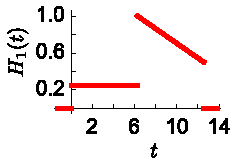
\includegraphics[scale=1]{figures/jumpop_drive_edited_v2.pdf}
		\caption{\label{fig:jumpop-trace:drive}Piecewise analytical drive.}
	\end{subfigure}%
	\begin{subfigure}[b]{0.7\linewidth}
		\centering
		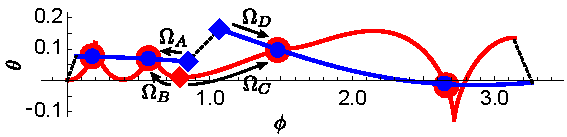
\includegraphics[scale=1]{figures/jumpop_trace_edited_v2.pdf}
		\caption{\label{fig:jumpop-trace:trajectory}Trajectories.}
	\end{subfigure}%
	\caption{\textbf{Effective Magnus trajectories under a piecewise analytical driving envelope.} \subcapref{fig:jumpop-trace:drive} An exemplary piecewise analytical driving envelope is shown. This envelope, with a total pulse duration of $t_d = 12.57$, exhibits non-analyticities at $t=0$ (turn-on time), $t=t_d/2$ and $t=t_d$ (turn-off time). The average drive strength over the total pulse duration is $\overline{H}_1 = 0.5$, such that the rotation induced by driving a two-level system with this particular pulse is $\theta_d = \overline{H}_1t_d/2=\pi$ in the rotating wave approximation. \subcapref{fig:jumpop-trace:trajectory} The axes on this figure represent the spherical latitude $\theta$ and longitude $\phi$ on a rotated Bloch sphere, i.e. a Bloch sphere that has the state $\ket{+}$ as its north pole. In particular, $\theta = 2 \arccos\left(\left|\braket{\psi|+}\right|\right) - \pi/2$ and $\phi = \arg\left(\braket{\psi|-}\right) - \arg\left(\braket{\psi|+}\right)$. The evolution (red line) of a system initially in the $\ket{0}$ state, driven by a sinusoidal signal with an envelope as given in Figure~\subref{fig:jumpop-trace:drive}, is obtained through numerical integration. In addition, the stroboscopic Magnus trajectory of order $1/\omega^2$ (blue lines) is plotted. The actual and stroboscopic trajectories approximately coincide every $t_c=\pi / \omega$, starting at $t_0 = \alpha_0/\omega$ (red, blue dots). At each non-analytical point in the driving envelope, the stroboscopic trajectory shows a ``jump'' (dashed lines). For the second discontinuity, at $t = t_d/2$, the corresponding point on each trajectory is indicated (diamond). Around this discontinuity, generators of evolution operators along several sections of the actual and the stroboscopic trajectories are marked ($\Omega_i$) and expanded upon in the main text. Relevant parameters are $\omega = 1$, $\alpha_0 = 0.9$. }
	\label{fig:jumpop-trace}
\end{figure}

Figure~\ref{fig:jumpop-trace} illustrates this situation. A system, initially in the state $\ket{\psi_\real(t=0)}=\ket{0}$, is driven using a particular driving envelope, shown in Figure~\ref{fig:jumpop-trace:drive}, that exhibits discontinuities at the turn-on time $t=0$ and the turn-off time $t_d$, in addition to a discontinuity at $t_j = t_d/2$. For this discussion, we focus on the discontinuity at $t_j$ and define $E_l(t)$ ($E_r(t)$) as the part of the envelope function to the left (right) of $t_j$. 

Our goal now is to find an effective trajectory $\ket{\psi_{\eff}(t)}$ that 
\begin{enumerate*}[label=(\alph*)]
	\item stroboscopically coincides with the actual trajectory, and
	\item evolves corresponding to $E_l(t)$ for $t<t_j$ and to $E_r(t)$ for $t>t_j$.
\end{enumerate*} 
The second condition fixes the shape of the effective trajectory sections $\ket{\psi_{\eff}(t)}_l $ and $\ket{\psi_{\eff}(t)}_r$ to the left and right of $t_j$, while the first condition fixes the positions of these sections. Although the real trajectory is necessarily continuous everywhere under unitary evolution, in general, the combined effective trajectory is not continuous at $t_j$, as shown in Figure~\ref{fig:jumpop-trace:trajectory}. We describe this discontinuity with an ``impulse operator'', which will be subject of the next section.

\subsection{The impulse operator}
\newcommand{\evolexp}[1]{e^{#1}}
The impulse operator $\Omega_j$ is defined as the generator of the unitary operator that rotates the endpoint $\ket{\psi_{\eff}(t_j)}_l$ of the effective trajectory section to the left of $t_j$ to the starting point $\ket{\psi_{\eff}(t_j)}_r$ of the section to the right of $t_j$. That is,
\begin{align}
	\ket{\psi_{\eff}(t_j)}_r = \evolexp{\Omega_j} \ket{\psi_{\eff}(t_j)}_l.
\end{align}
From Figure~\ref{fig:jumpop-trace:trajectory}, we see that
\begin{align}
	\evolexp{\Omega_j} = (\evolexp{\Omega_D})^{-1} \evolexp{\Omega_C} (\evolexp{\Omega_B})^{-1} \evolexp{\Omega_A} = \evolexp{-\Omega_D} \evolexp{\Omega_C} \evolexp{-\Omega_B} \evolexp{\Omega_A},
	\label{eq:omega_j-defintion}
\end{align}
where $\Omega_i, i \in \{A,B,C,D\}$ are all generators of unitaries that describe the evolution between certain points on the actual and effective trajectories. In particular,
\begin{alignat}{2}
	&\ket{\psi_\eff(t_0)}_l &&= \evolexp{\Omega_A} \ket{\psi_\eff(t_j)}_l \label{eq:omega_A-definition} \\
	&\ket{\psi_\real(t_0)} &&= \evolexp{\Omega_B} \ket{\psi_\real(t_j)} \label{eq:omega_B-definition} \\
	&\ket{\psi_\real(t_0+t_c)} &&= \evolexp{\Omega_C} \ket{\psi_\real(t_j)} \label{eq:omega_C-definition} \\
	&\ket{\psi_\eff(t_0+t_c)}_r &&= \evolexp{\Omega_D} \ket{\psi_\eff(t_j)}_r. \label{eq:omega_D-definition}
\end{alignat}
The definition of the effective trajectory requires that $\ket{\psi_\eff(t_0)}_l = \ket{\psi_\real(t_0)}$ and $\ket{\psi_\eff(t_0+t_c)}_r = \ket{\psi_\real(t_0+t_c)}$. Equation (\ref{eq:omega_j-defintion}) then follows immediately from definitions (\ref{eq:omega_A-definition})-(\ref{eq:omega_D-definition}) and the stroboscopic coincidence condition.

We use explicit Magnus expansions (as per Daniel's definition) to express the four $\Omega_i$'s. For example,
\begin{align}
	\Omega_A = M\left[H_{\eff,l}(t), t_0, t_j\right].
	\label{eq:Omega_A-explicit-ME}
\end{align}
For this particular explicit Magnus expansion, we substitute $E(t)$ by a Taylor expansion of $E_l(t)$ around $t_j$. For the other explicit Magnus expansions we also substitute $E(t)$ by a Taylor expansion around $t_j$ of $E_l(t)$ or $E_r(t)$ appropriately. Finally, we construct an expression for $\Omega_j$ by repeated application of the Baker-Campbell-Hausdorff (BCH) formula to equation (\ref{eq:omega_j-defintion}).

\subsection{The impulse operator as a power series in $1/\omega$}
In principle, the impulse operator introduced in the previous section is exact if the relevant Magnus and Taylor expansions and the BCH formula are treated up to infinite order. In this section we will discuss how to calculate the impulse operator up to finite order $k$ in $1/\omega$. 

As a first step, we express the two relevant times in the problem, $t_0$ and $t_j$, relative to the time scale $1/\omega$ of the power series by introducing the angle-like quantities $\alpha_0 = \omega t_0$ and $\alpha_j = \omega t_j$. We then calculate explicit Magnus expansions for all four $\Omega_i$'s (cf. eq. (\ref{eq:Omega_A-explicit-ME})) up to the desired order $k$ in $1/\omega$, using the method detailed in Daniel's notes. Noting that the impulse operator needs to be dimensionless, a similar dimensional argument as applied in Daniel's note leads us to the conclusion that the highest relevant order of the envelope Taylor expansions is $k-1$.

Subsequently, we note that the substitutions $t_0 = \alpha_0/\omega$ and $t_j = \alpha_j/\omega$ render all integral bounds in the Magnus expansion proportional to $1/\omega$, such that the integrals and therefore the $\Omega_i$'s themselves become proportional to $1/\omega$. This implies that an $n$-th order nested commutator of $\Omega_i$'s is proportional to $1/\omega^{n+1}$. Therefore, the highest order of nested commutators in the BCH formula we need to take into account is $k-1$.

After putting this machinery to work, we arrive at a power series for the impulse operator $\Omega_j$. The first three terms are given by
\begin{alignat}{3}
	&\Omega_j &&=\,\,&&\sum_{i=0}^\infty \frac{1}{\omega^i} \Omega_j^{(i)}, \\
	&\Omega_j^{(0)} && = &&0, \label{eq:Omega_j-ww-0} \\
	&\Omega_j^{(1)} && = &&i\frac{\sin(\alpha_j - \alpha_0)}{4}(E_r-E_l)\cdot(\cos(\phi+\alpha_0+\alpha_j)\sx - \sin(\phi+\alpha_0+\alpha_j)\sy), \label{eq:Omega_j-ww-1} \\
	&\Omega_j^{(2)} && = &&-i\frac{\sin(\alpha_j - \alpha_0)}{32} \times \label{eq:Omega_j-ww-2} \\
	& && && \Big( 4\Delta(E_r - E_l) \cdot \big( \cos(\phi+\alpha_0+\alpha_j) \sx + \sin(\phi+\alpha_0+\alpha_j) \sy \big)\nonumber \\
	& && && + 4(\dot{E}_r - \dot{E}_l) \cdot \big( \sin(\phi+\alpha_0+\alpha_j) \sx - \cos(\phi+\alpha_0+\alpha_j) \sy \big) \nonumber \\
	& && && + (E_r^2-E_l^2) \cdot \big(\cos(\alpha_j - \alpha_0) - 2\cos(2\phi+\alpha_0+\alpha_j)\big)\sz \Big), \nonumber 
\end{alignat}
where $E_{r,l}$ and $\dot{E}_{r,l}$ are shorthand for the Taylor coefficients $E_{r,l}(t_j)$ and $\dot{E}_{r,l}(t_j)$ respectively.

\subsubsection{Final and initial impulse operators}
The impulse operator formalism is also capable of describing the discontinuity in the effective trajectory during a non-analytical turn-on or turn-off of the driving field. In this case, either $E_l(t)$ or $E_r(t)$ is identically zero and the expressions (\ref{eq:Omega_j-ww-0})-(\ref{eq:Omega_j-ww-2}) simplify accordingly. 

In addition, for computational simplicity when calculating higher order initial or final impulse operators, we can simplify eq. (\ref{eq:omega_j-defintion}) considerably. For example, if we're interested in the turn-on discontinuity at $t=0$, for $t<0$ the system Hamiltonian is given by 
\begin{align}
	\label{eq:H-nodrive}
	\matr{H}_\real(t) = \frac{\Delta}{2}\sz.
\end{align}
This Hamiltonian is constant and can be represented exactly in the effective Hamiltonian formalism, even at the lowest (zeroeth) order in $1/\omega$. Therefore, we can take $\matr{H}_\eff(t) = \matr{H}_\real(t)$ for $t<0$. Then it follows that $\Omega_A = -i\matr{H}_\eff (t_0 - t_j) = -i\matr{H}_\real (t_0 - t_j) = \Omega_B$ and
\begin{align}
	\evolexp{\Omega_j} = \evolexp{-\Omega_D}\evolexp{\Omega_C}.
\end{align}
A similar argument can be made for the turn-off discontinuity. Note that the ``turn-off impulse operator'' can also be used at any point in time $t$ to calculate the transformation from the effective trajectory to the real trajectory at that time.

% \begin{alignat}{3}
% 	&\Omega_2(t,t_0) &&= \phantom{-} \frac{1}{2}\int_{t_0}^t \mathrm{d}t_1 \int_{t_0}^{t_1} \mathrm{d}t_2 \big[ && -iH(t_1), -iH(t_2) \big] \nonumber \\
% 	& &&= - \frac{1}{2}\int_{t_0}^t \mathrm{d}t_1 \int_{t_0}^{t_1} \mathrm{d}t_2 \big[ &&\frac{E(t_1)}{4}\left( (1 + \cos(2 \omega t_1)) \sx - \sin(2 \omega t_1) \sy \right), \nonumber \\ 
% 	& && &&\frac{E(t_2)}{4}\left( (1 + \cos(2 \omega t_2)) \sx - \sin(2 \omega t_2) \sy \right) \big]
% \end{alignat}

\newpage 

\section{The truncated Magnus expansion}
\label{sec:magnus-expansion}
The Magnus expansion\supercite{Magnusexponentialsolutiondifferential1954,harris_average_2007,BlanesMagnusexpansionits2009,BlanespedagogicalapproachMagnus2010} for the time evolution under Hamiltonian $H(t)$ is defined as
\begin{alignat}{2}
	&\Omega(t,t_0) &&= \sum_{n=1}^\infty \Omega_n(t,t_0),\\
	&\Omega_1(t,t_0) &&= \int_{t_0}^t \mathrm{d}t_1 \tilde{H}(t_1),\label{eq:omg-1}\\
	&\Omega_2(t,t_0) &&= -\frac{1}{2}\int_{t_0}^t \mathrm{d}t_1 \left[ \Omega_1(t_1,t_0), \tilde{H}(t_1) \right] = \frac{1}{2}\int_{t_0}^t \mathrm{d}t_1 \int_{t_0}^{t_1} \mathrm{d}t_2 \left[ \tilde{H}(t_1), \tilde{H}(t_2) \right] \label{eq:omg-2},
\end{alignat}
where $\tilde{H}(t) = -i / \hbar H(t)$. In the remainder of these notes, natural units with $\hbar = 1$ will be used.

We use this series to approximate the trajectory of a two-level qubit driven by an oscillating signal proportional to $\matr{\sigma}_x$ in the lab frame. To this end, we use the following rotating frame Hamiltonian:
\begin{align}
	\label{eq:H-drive}
	\matr{H}(t) = \frac{E(t)}{4}\left( \sx + \cos(2 \omega t) \sx - \sin(2 \omega t) \sy \right),
\end{align}
where for now we have set the detuning $\Delta$ and phase offset $\phi$ of the drive both to zero.

\subsection{First order Magnus expansion}
Initially, we restrict ourselves to the first order Magnus term, which is equivalent to the rotating wave approximation for constant drive. We begin by studying the case of linear drive, given by
\begin{align}
	E(t) = E_0 + E_1 t.
\end{align}
We then integrate equation (\ref{eq:omg-1}) over a full period $t_c = \pi / \omega$ of the drive Hamiltonian (\ref{eq:H-drive}), starting from $t_0$:
\begin{align}
	i \Omega_1(t_0+t_c,t_0) = &\int_{t_0}^{t_0+t_c} \frac{E(t)}{4}\left( \sx + \cos(2 \omega t) \sx - \sin(2 \omega t) \sy \right) \, \mathrm{d}t \nonumber \\
	= &\int_{t_0}^{t_0+t_c} \frac{E(t)}{4} \sx \, \mathrm{d}t + \int_{t_0}^{t_0+t_c} \frac{E(t)}{4} (\cos(2 \omega t) \sx - \sin(2 \omega t) \sy) \, \mathrm{d}t \nonumber \\
	= &\frac{E_0 t_c  + E_1 (t_0 t_c + t_c^2 / 2)}{4} \sx + \frac{E_1 t_c \sin(2 \omega t_0)}{8\omega} \sx + \frac{E_1 t_c \cos(2 \omega t_0)}{8\omega} \sy \nonumber \\
	= &t_c\frac{E_0 + E_1 t_0}{4} \sx + t_c^2 \frac{E_1}{8} \sx + \frac{t_c}{\omega} \left( \frac{E_1 \sin(2 \omega t_0)}{8} \sx + \frac{E_1 \cos(2 \omega t_0)}{8} \sy \right) \nonumber \\
	= &t_c\left[ \frac{E_0 + E_1 t_0}{4} \sx + \frac{E_1}{8 \omega} \left( \pi \sx + \sin(2 \omega t_0) \sx + \cos(2 \omega t_0) \sy \right) \right] \label{eq:evexp-order-1}
\end{align}
The first term of this evolution operator exponent,
\begin{align}
	\label{eq:evexp-rwa-constant-term}
	t_c \frac{E_0 + E_1 t_0}{4} \sx = t_c \frac{E(t_0)}{4} \sx,
\end{align}
can be understood as the rotating wave evolution over a period $t_c$ with constant drive given by the value of the driving envelope at the beginning of the evolution period $E(t_0)$. The second term,
\begin{align}
	\label{eq:evexp-rwa-linear-term}
	t_c^2\frac{E_1}{8}\sx=t_c\frac{\pi E_1}{8 \omega}\sx,
\end{align}
can still be understood in the rotating wave picture as the extra rotation brought about by the (linear) increase in driving strength during the evolution interval $t_c$. Keeping in mind that $t_c = \pi / \omega$, the effect of this term decreases if $\omega$ increases; i.e. the driving signal has less time to increase within one evolution interval. 

The final two terms in equation (\ref{eq:evexp-order-1}),
\begin{align}
	t_c \frac{E_1}{8 \omega} \left( \sin(2 \omega t_0) \sx + \cos(2 \omega t_0) \sy \right),
\end{align}
can no longer be understood in the rotating wave approximation. These terms constitute an average of the effect of the counter-rotating wave over a single evolution interval $t_c$, which is exactly the period of the counter-rotating wave. In the case of constant drive, i.e. $E_1 = 0$, this effect averages out to zero, but if the drive increases during the evolution interval, a non-zero average is obtained. The resulting ``average counter-wave rotation axis'' lies in the $x-y$ plane and has a constant magnitude, while the direction is determined by the start of the evolution interval $t_0$, as illustrated in Figure~\ref{fig:avg-crwave-rotation-lindrive}.

\begin{figure}[tb]
	\centering
	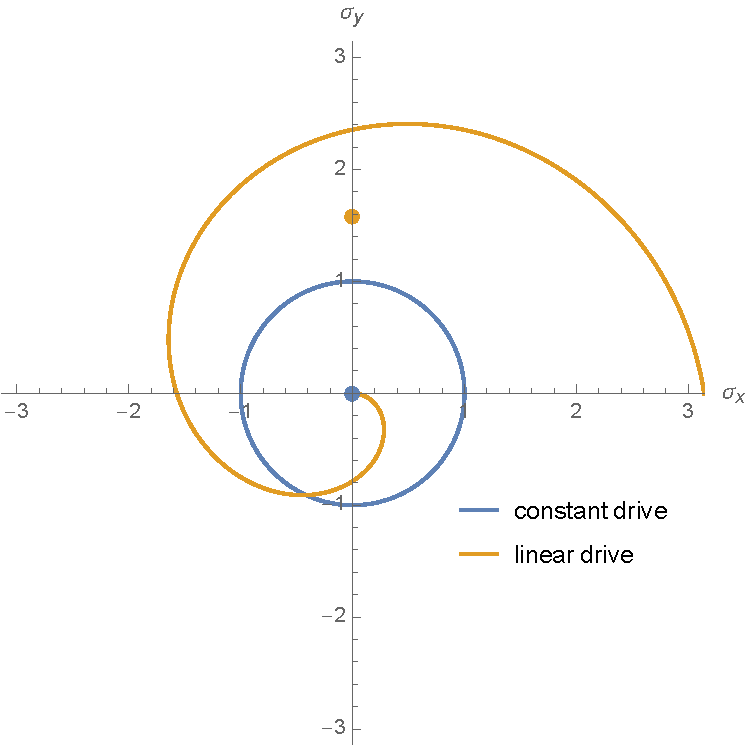
\includegraphics[width=0.5\textwidth]{figures/avg-CR-wave-rotation-lindrive.pdf}
	\caption{\textbf{Effect of the counter-rotating wave in the first order Magnus expansion.} The $\sx$ and $\sy$ projections of the counter-rotating wave contribution, $E(t) \left[\cos(2 \omega t) \sx + \sin(2 \omega t) \sy \right]$, are traced for $t \in [t_0,t_0+t_c]$ with $t_0=0$. Trajectories are shown both for constant drive $E(t) = 1$ and for a linearly increasing drive $E(t)=(t-t_0)$. The average projections are indicated with a dot. For constant drive, it can be seen that the average projection is zero, while for linear drive, the average is non-zero and directed $\pi/2$ radians from the initial (and final) projection. Choosing a different $t_0$ has the effect of rotating the trajectories and still leaves a non-zero average of equal magnitude in the linear drive case.}
	\label{fig:avg-crwave-rotation-lindrive}
\end{figure}

\subsubsection{Effective Hamiltonian}
Let's see if we can find an effective Hamiltonian that corresponds to (\ref{eq:evexp-order-1}). Per the procedure described in Daniel's notes, we proceed order by order of $1 / \omega$, such that $H_{eff}^{(m)}=\sum_{n=0}^m (1 / \omega)^n h_n$, where each $h_n$ may not depend explicitly on $t$ or $\omega$ and occurences of $t_0$ in (derivatives of) $H_1(t_0)$ are promoted to the instantaneous time $t$. We start with the trivial order $1 / \omega^0 = 1$. In this case, $h_0$ is given by 
\begin{align}
	h_0 = \left[\frac{E(t_0)}{4}\sx\right]_{t_0 \to t} = \frac{H(t)}{4}\sx. \label{eq:heff-order-0}
\end{align}
For the next order $1 / \omega^1$ we use the iterative relation 
\begin{align}
	h_{n+1} = C[\bar{H}(t_0), 1 / \omega, n+1] - C[\bar{H}_{eff}^{(n)}(t_0),1/\omega,n+1].
\end{align}
The first term is readily extracted from (\ref{eq:evexp-order-1}) and equal to
\begin{align}
	C[\bar{H}(t_0), 1 / \omega, 1] = \frac{E_1}{8 \omega} \left( \pi \sx + \sin(2 \omega t_0) \sx + \cos(2 \omega t_0) \sy \right).
\end{align}
The second term is obtained by calculating the Magnus expansion of (\ref{eq:heff-order-0}) up to first order in $1 / \omega$. Noting that $h_0$ is proportional to $\sx$ for all times and $[h_0(t_1),h_0(t_2)] = 0$ for all $t_1, t_2$, the first order Magnus expansion is exact and given by
\begin{align}
	\bar{H}_{eff}^{(0)}(t_0) = \left[ \frac{E(t_0)}{4} + \frac{E_1}{8 \omega} \pi \right] \sx.
\end{align}
Therefore,
\begin{align}
	C[\bar{H}_{eff}^{(0)}(t_0),1/\omega,1] = \frac{E_1}{8 \omega} \pi \sx,
\end{align}
leaving us with
\begin{align}
	h_1 = \frac{E_1}{8 \omega} \left( \sin(2 \omega t_0) \sx + \cos(2 \omega t_0) \sy \right).
\end{align}

Let's see if taking the Magnus expansion of this effective Hamiltonian indeed matches the ME of the real Hamiltonian over an interval $t_c$. As per the notebook `linear\_drive\_manual\_integration.nb' it does, up to first order! There is however a third order term (and higher order terms) that explains the deviation of the trajectory of the effective Hamiltonian from the stroboscopic evolution given by repeated application of $\exp[-i t_c \bar{H}(t_0 + k t_c)]$ with increasing $k$, as observed in numerical simulations for large driving strengths.

\subsection{Second order Magnus expansion}
We now continue by investigating the second order term in the Magnus expansion, given by (\ref{eq:omg-2}), to gain some intuition. We first focus on rewriting the commutator in the integrand:
\begin{alignat}{1}
	&\frac{1}{2}\big[ \tilde{H}(t_1), \tilde{H}(t_2) \big] = \frac{1}{2}\left[ -iH(t_1), -iH(t_2) \right] = - \frac{1}{2}\left[ H(t_1), H(t_2) \right] \nonumber \\
	&= -\frac{E(t_1)E(t_2)}{32} \big[ \left( (1 + \cos(2 \omega t_1)) \sx - \sin(2 \omega t_1) \sy \right), \left( (1 + \cos(2 \omega t_2)) \sx - \sin(2 \omega t_2) \sy \right) \big] \nonumber \\
	&= \frac{E(t_1)E(t_2)}{32} \Big( (1 + \cos(2 \omega t_1))\sin(2 \omega t_2) \left[  \sx, \sy \right] + \sin(2 \omega t_1) (1 + \cos(2 \omega t_2)) \left[\sy,\sx\right] \Big) \nonumber \\
	&= i \frac{E(t_1)E(t_2)}{32} \Big( (1 + \cos(2 \omega t_1))\sin(2 \omega t_2) - \sin(2 \omega t_1) (1 + \cos(2 \omega t_2)) \Big) \sz \label{eq:o2-itgd-expandedform} \\
	&= -i\frac{E(t_1)E(t_2)}{4} \cos(\omega t_1) \cos(\omega t_2) \sin(\omega(t_1 - t_2)) \sz \label{eq:o2-itgd-condensedform}.
\end{alignat}
A few important qualitative properties of the integrand and thus of the second order Magnus expansion term can be inferred from (\ref{eq:o2-itgd-condensedform}). Firstly, containing only the commutator $[\sx,\sy]$, the integrand is proportional to $\sz$ and represents the second order ``composition effect'' of non-commuting rotations around different axes in the $x-y$ plane. Furthermore, for $t_1 = t_2$ the final sine factor is zero, as is to be expected for the commutator at equal times.

% After plugging in the linear drive envelope, we arrive at the integrand
% \begin{align}
% 	-i\frac{(E_0 + E_1 t_1)(E_0 + E_1 t_2 )}{4} \cos(\omega t_1) \cos(\omega t_2) \sin(\omega(t_1 - t_2)) \sz.
% \end{align}
Noting that this integrand is to be doubly integrated over $t_1$ and $t_2$, it is wise to make the integrand separable into factors only depending on $t_1$ or $t_2$. This yields the integrand
\begin{alignat}{2}
	& &&\frac{-iE(t_1)E(t_2)}{4} \cos(\omega t_1) \cos(\omega t_2) \left( \sin(\omega t_1)\cos(\omega t_2) - \cos(\omega t_1)\sin(\omega t_2) \right) \sz \nonumber \\
	&= &&\frac{-i}{8} \sz \left( E(t_1) \sin(2 \omega t_1) E(t_2) \cos(\omega t_2)^2 \right) + \frac{i}{8} \sz \left( E(t_1) \cos(\omega t_1)^2 E(t_2) \sin(2 \omega t_2) \right). \label{eq:o2-itgd-separable}
\end{alignat}
We proceed by performing the inner integrals over $\mathrm{d}t_2$, resulting in
\begin{alignat}{2}
	&\int_{t_0}^{t_1} \mathrm{d}t_2\, E(t_2) \cos(\omega t_2)^2 &&= \int_{t_0}^{t_1} \mathrm{d}t_2\, (E_0 + E_1 t_2) \cos(\omega t_2)^2 \nonumber \\
	& &&= \frac{1}{4}(t_1 - t_0)\left( E(t_0) + E(t_1) \right) \nonumber \\
	& &&+ \frac{1}{4\omega} \left( E(t_1) \sin(2 t_1 \omega) - E(t_0) \sin(2 t_0 \omega) \right) \nonumber  \\
	& &&+ \frac{E_1}{8 \omega^2} \left( \cos(2 t_1 \omega) - \cos(2 t_0 \omega) \right) \label{eq:o2-itgd-inner1}\\
	&\int_{t_0}^{t_1} \mathrm{d}t_2\, E(t_2) \sin(2 \omega t_2) &&= \int_{t_0}^{t_1} \mathrm{d}t_2\, (E_0 + E_1 t_2) \sin(2 \omega t_2) \nonumber \\
	& &&= \frac{1}{2 \omega} \left( E(t_0) \cos(2 t_0 \omega) - E(t_1) \cos(2 t_1 \omega) \right) \nonumber \\
	& &&+ \frac{E_1}{4 \omega^2} \left( \sin(2 t_1 \omega) - \sin(2 t_0 \omega) \right). \label{eq:o2-itgd-inner2}
\end{alignat}
Plugging (\ref{eq:o2-itgd-inner1}) and (\ref{eq:o2-itgd-inner2}) into the integral of (\ref{eq:o2-itgd-separable}) over $\mathrm{d}t_2 \in [t_0,t_1]$ yields
\begin{alignat}{2}
	&-\frac{i}{8} \sz  E(t_1) \sin(2 \omega t_1) \Big( && \frac{1}{4}(t_1 - t_0)\left( E(t_0) + E(t_1) \right) \nonumber \\
	& &&+ \frac{1}{4\omega} \left( E(t_1) \sin(2 t_1 \omega) - E(t_0) \sin(2 t_0 \omega) \right) \nonumber  \\
	& &&+ \frac{E_1}{8 \omega^2} \left( \cos(2 t_1 \omega) - \cos(2 t_0 \omega) \right) \Big)  \nonumber \\
	&+ \frac{i}{8} \sz  E(t_1) \cos(\omega t_1)^2 \Big( &&\frac{1}{2 \omega} \left( E(t_0) \cos(2 t_0 \omega) - E(t_1) \cos(2 t_1 \omega) \right) \nonumber \\
	& &&+ \frac{E_1}{4 \omega^2} \left( \sin(2 t_1 \omega) - \sin(2 t_0 \omega) \right) \Big),
\end{alignat}
which thankfully can be simplified (by Mathematica, not by me...) to
\begin{align}
	&\frac{i}{16}\sz E(t_1)\cos(\omega t_1) (t_0-t_1)(E(t_0) + E(t_1))\sin(\omega t_1) \nonumber \\
	&-\frac{i}{16 \omega} \sz E(t_1)\cos(\omega t_1)(E(t_1)\cos(\omega t_1) -E(t_0) \cos(\omega(2 t_0 - t_1))) \nonumber \\
	&+\frac{i E_1}{32 \omega^2}\sz E(t_1) \cos(\omega t_1) (\sin(\omega t_1) - \sin(\omega (2 t_0-t_1))).
\end{align}
Finally, we calculate the second order Magnus exponent term by integrating the previous expression with respect to $\mathrm{d}t_1$ over an evolution interval $t_c$, starting from $t_0$:
\begin{align}
	\frac{i}{t_c}\Omega_2(t_0+t_c,t_0) &= \frac{E(t_0)^2}{32 \omega} \sz (1 - 2 \cos(2 \omega t_0)) \nonumber \\
	&+\frac{E_1 E(t_0)}{32 \omega^2} \sz \left( \pi - 2\pi \cos(2 \omega t_0) - 3 \sin(2 \omega t_0)\right) \nonumber \\
	&+\frac{E_1^2}{384 \omega^3} \sz \left( 3 + 4\pi^2 + (18 - 6 \pi^2) \cos(2 \omega t_0) + 18\pi\sin(2 \omega t_0)\right) \label{eq:o2-term}.
\end{align}
Direct calculation of the second order Magnus term using Daniel's scripts yields the same expression, which is comforting.

The first term of (\ref{eq:o2-term}) represents the Bloch-Siegert shift and is the only term that survives for a constant drive with $E_1 = 0$. For $t_0 = k t_c$, we can understand the second term and the parts of third term that contain $\pi^2$ as the increase in Bloch-Siegert shift during the evolution interval $t_c$, similar to (\ref{eq:evexp-rwa-linear-term}).

Noting that the expressions and integrals become increasingly complicated for higher order Magnus terms, we stop here with the manual integration and intuitive interpretation of the Magnus terms.

\newpage


\printbibliography
	
\end{document}